\subsection{Automated Identification of Uniqueness for Generating Test Names}
\label{sec:uniquness-approach}

As the second component towards generating descriptive test names, I built an automated approach to extract unique attributes of unit tests based on the results of previous component.
%
To check the consistency of the approach, I further conducted an empirical evaluation on a set of randomly chosen tests from various open-source projects on Github by using a working prototype of it.
%
The conclusion of the evaluation shows the approach is consistent with human judgment and useful for future name generation techniques.


\subsubsection{Description of the Approach}

\Cref{fig:overview} presents a high-level overview of our approach for automatically identifying the unique attributes of tests.
%
As the figure shows, the approach takes a unit test and its sibling tests as input and identifies a set of unique attributes for the given test in two main steps.
%
Step~1 is to extract attributes from the test and its siblings.
%
The attributes are extracted using information matchers that correspond to the various selective codes identified as part of the empirical study in~\cref{sec:emp-study}.
%
Step~2 is to determine whether the extracted attributes are the portions of the test that make it unique from its siblings.
%
If the attributes do make it unique, the approach proceeds to output the current attributes for the test.
%
However, if the attributes are not unique, the approach returns to Step~1 and extracts a different set of attributes.
%
The order in which Step~1 extracts attributes is based on the results of the empirical study; attributes that correspond to selective codes that are more likely to be what makes a test unique are tried before attributes that correspond to codes that are less likely to be unique.
% 
The loop between Step~1 and Step~2 proceeds until either a set of unique attributes are found or, if none of the attributes uniquely identifies the test, the approach terminates with an empty set of attributes.
%
Additional details about each of the approach's steps are provided in the following subsections.


\begin{figure}[t]
\centering
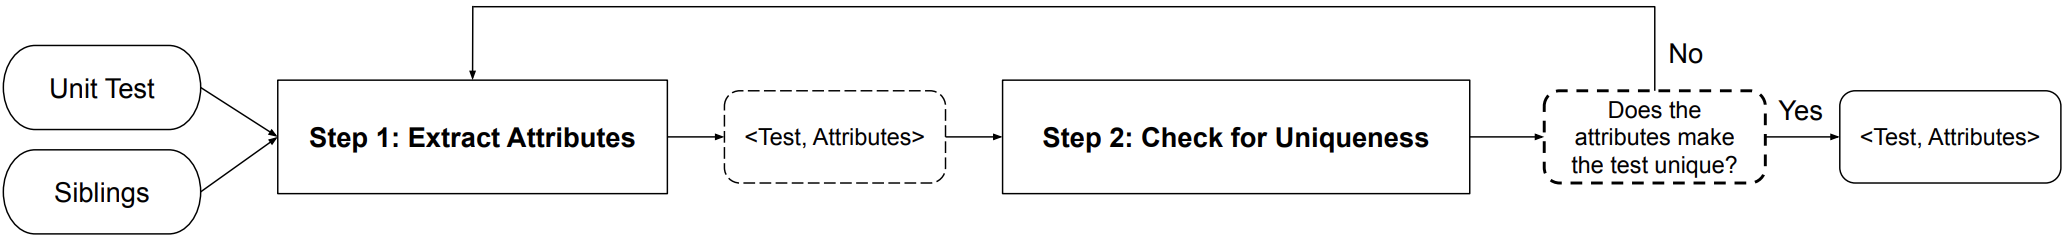
\includegraphics[width=\textwidth]{figures/ApproachOverview}
\caption{Overview of the automated approach.}
\label{fig:overview}
\end{figure}

\paragraph{Step 1: Extract Attributes}

\begin{figure}[t]
\centering
\begin{subfigure}[b]{0.5\textwidth}
\centering
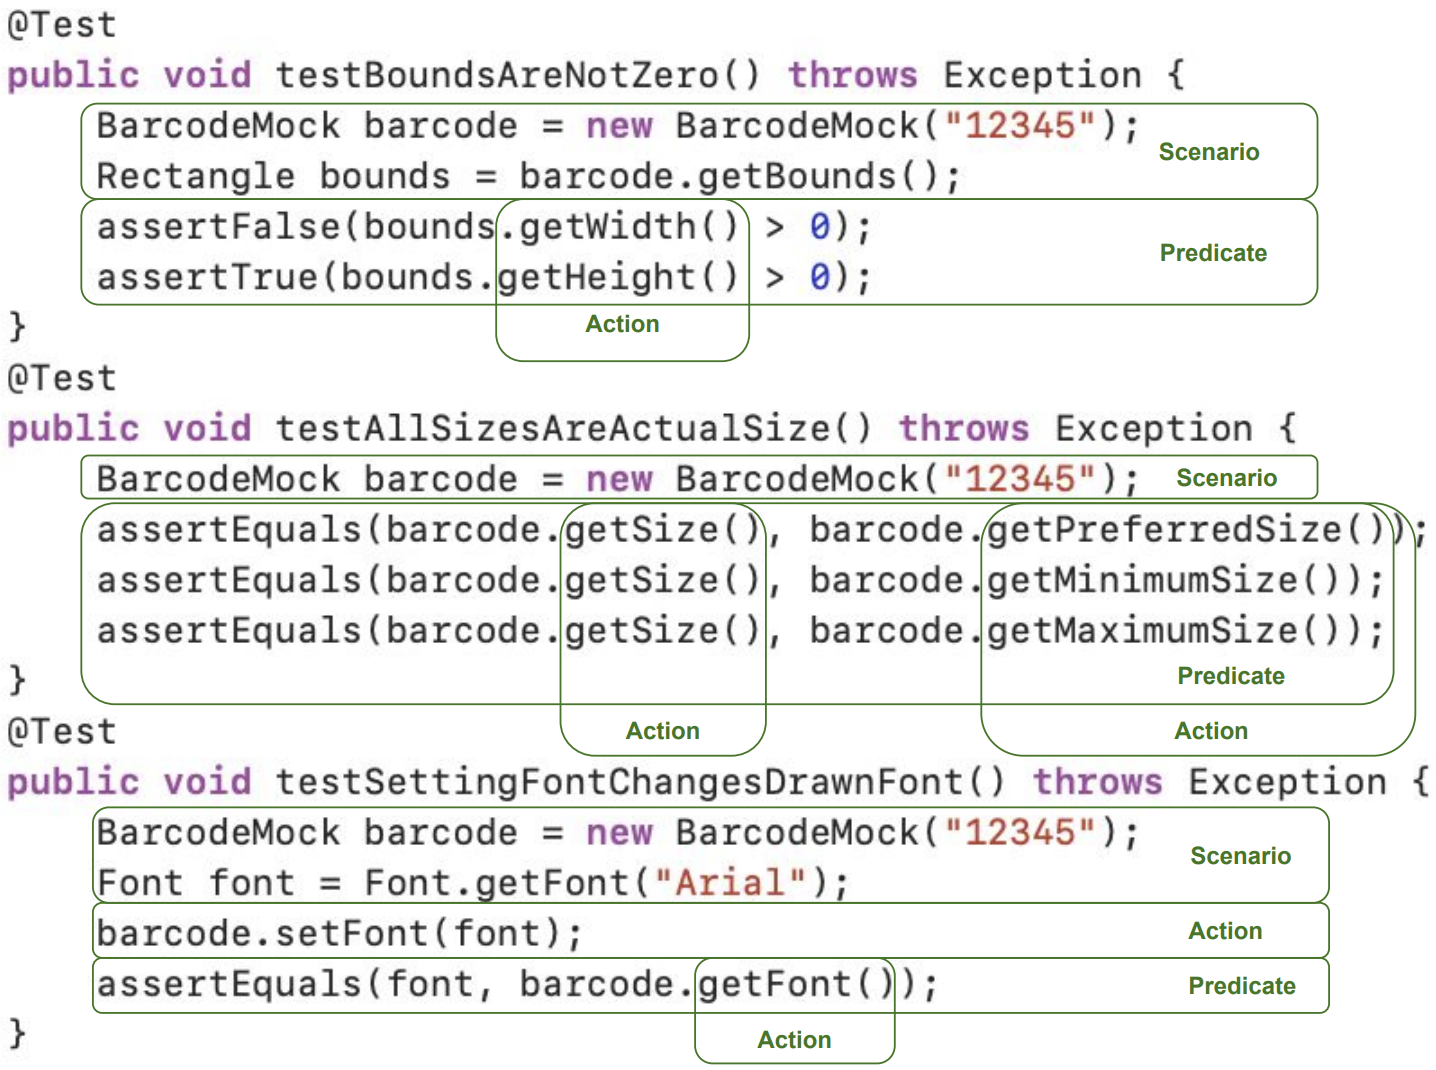
\includegraphics[scale=0.26]{figures/step1-1.png}
\caption{Matchers for top-level codes.}
\label{fig:matcher1}
\end{subfigure}\\
\vspace{0.2cm}
\begin{subfigure}[b]{0.5\textwidth}
\centering
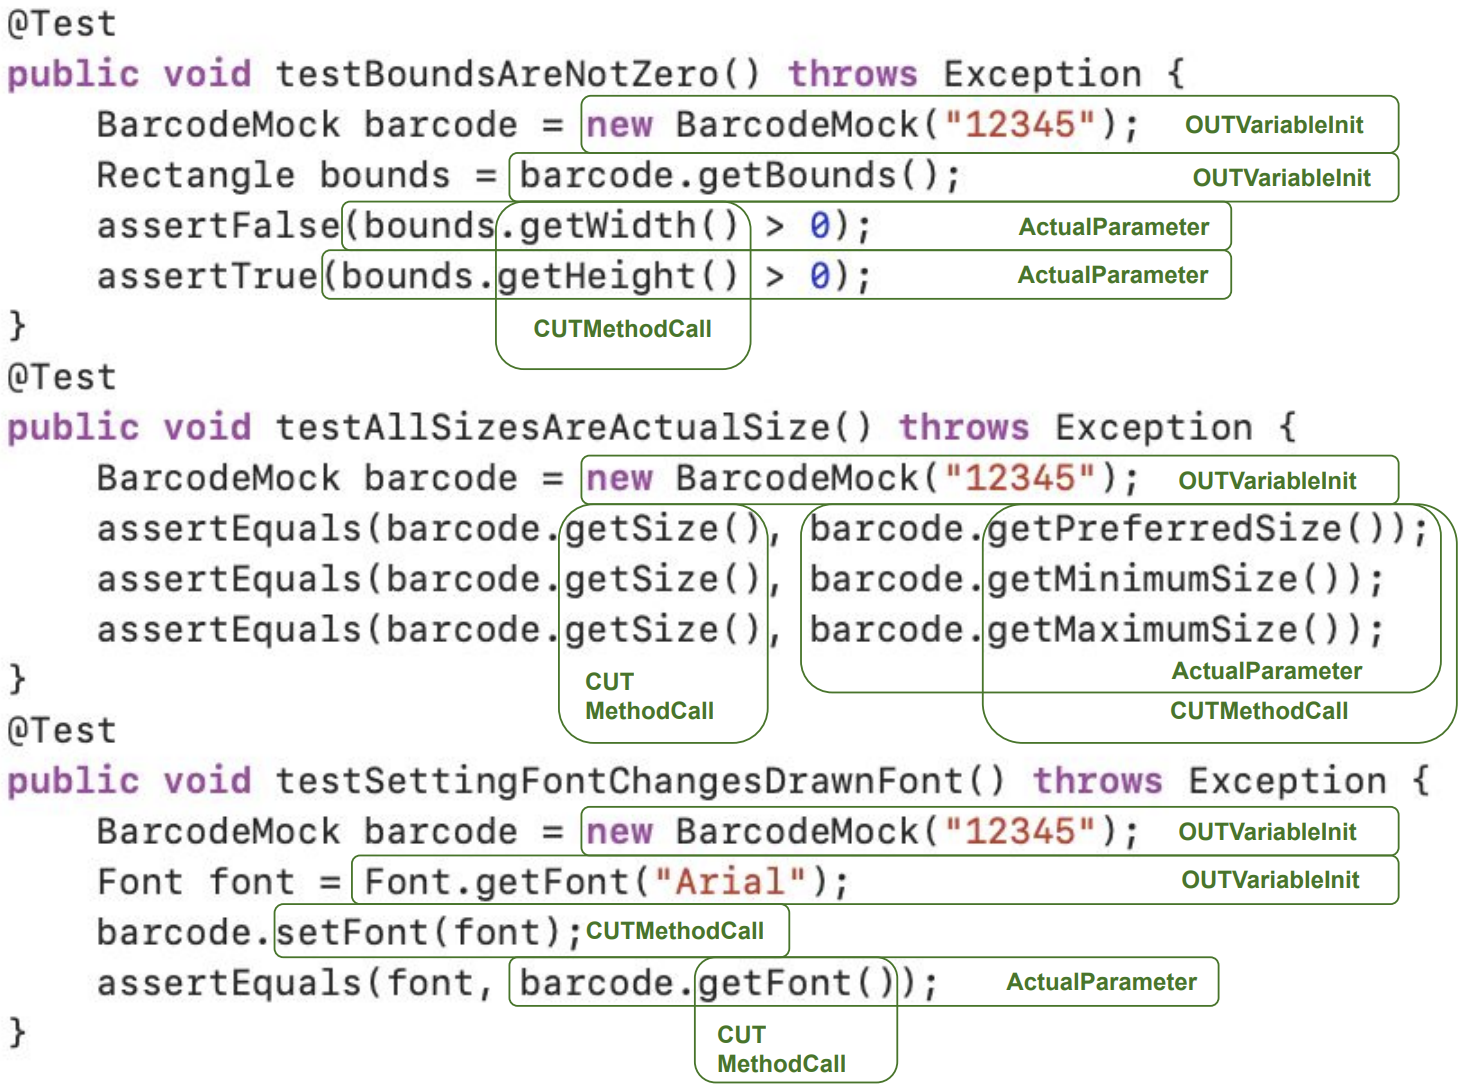
\includegraphics[scale=0.26]{figures/step1-2.png}
\caption{Matchers for secondary codes.}
\label{fig:matcher2}
\end{subfigure}
\caption{Example of information matchers.}
\label{fig:information-matcher}
\end{figure}

\begin{figure}[t]
\centering
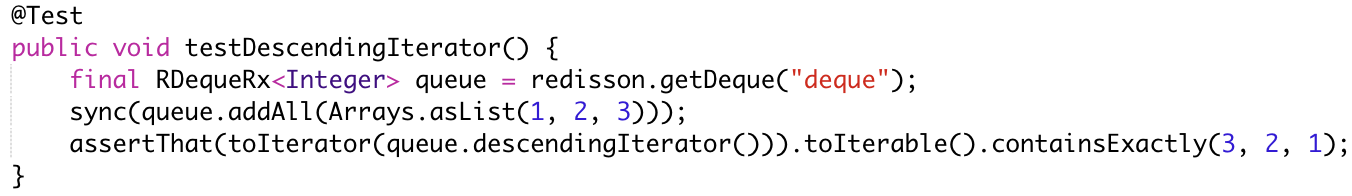
\includegraphics[scale=0.34]{figures/new-state-change.png}
\caption{Example of state-change methods.}
\label{fig:state-change}
\end{figure}


The goal of Step~1 is to extract attributes from each test that correspond to the information identified as part of the empirical study.
%
Essentially, this step is attempting to automate the manual process of identifying relevant portions of tests that was used in the study.
%
To do this, we built a set of information matchers, one for each selective code.
% 
These matchers extract attributes from the tests and produce a set of $\langle test,~attributes \rangle$ pairs, one for each give as input.
%
Each $\langle test,~attributes \rangle$ pair contains the test method and its corresponding attributes, and each test is identified by its name in the following examples.
%
This set of pairs are then used by the rest of the approach to generate a set of unique attributes.


Because the selective codes identify information at two levels (i.e., top-level and secondary codes), there are two corresponding types of information matchers.
%
Matchers for top-level codes are primarily concerned with segmenting tests into their various parts (i.e., action, predicate, scenario).
% 
The division of the test into blocks is implemented primarily via elimination.
%
First, the predicate matcher identifies calls to JUnit assertions and other predefined result-checking\slash verification methods.
%
For example in~\cref{fig:test2-proposal}, the call to the \texttt{verify} method is included as a predefined result-checking\slash verification method provided by the \texttt{Mockito} library.
%
Such calls become the predicate block.
% 
Note that calls to methods embedded inside assertions (e.g., to calculate the actual parameter) or nested after assertions (e.g., to change state of the unit test) are not included as part of the predicate block.
%
These calls are left for consideration by the matchers for the action and scenario.


Second, the action matcher identifies the remaining calls to CUT (i.e., class under test) and non-CUT methods jointly with their corresponding arguments.
%
Such calls become the action block.
%
Note that those nested calls to non-CUT methods that reside after assertions are not included as part of the action block.
%
These calls are left for consideration by the matchers for the scenario.
%
Finally, the scenario matcher identifies the OUT variable initializations, non-OUT variable initializations, control-flow variables, and calls to state-changing methods.
%
The combination of these code elements becomes the scenario block.
%
First, the scenario matcher first includes the calls to the state-changing methods of the test as part of the scenario block, which were previously excluded by the action matcher~\cite{zhang2016towards, wu2020pattern}.
%
For example in~\cref{fig:state-change}, for \texttt{testDescendingIterator} from \texttt{Redisson}, the call to the state-changing method is the first nested call after the assertion call: \texttt{toIterable}.
%
Then it also selects all of the OUT variable initializations, non-OUT variable initializations (i.e., differentiate from OUT by checking if it is used in the CUT method calls or assertions), and control-flow variables from the declaration and control-flow statements in the test.


As an example of how the high-level matchers work, consider the example shown in \cref{fig:information-matcher} which consists of three tests from Barbecue's \texttt{BarcodeTest} class.
% 
In the example, \texttt{testSettingFontChangesDrawnFont} will be the target test and the other two will be the the target's siblings.
%
The target test's predicate, action, and scenario are identified as follows:
%
The matcher for the \texttt{Predicate} code marks all of the JUnit assertions in the test body as the predicate block (i.e., one statement circled in green, tagged with \texttt{Predicate}).
%
Next, the matcher for the \texttt{Action} code marks all of the CUT method calls in the test body as the action block (i.e., one full and one partial statements circled in green, tagged with \texttt{Action}).
%
Finally, the matcher for the \texttt{Scenario} code marks all of the OUT variable initializations in the test body as the scenario block (i.e., two statements circled in green, tagged with \texttt{Scenario}).


Matchers for secondary codes are primarily concerned with identifying specific features within the blocks identified by the top-level information matchers.
%
To accomplish this, these secondary matchers select the corresponding code element from the action, predicate, or scenario block.
%
Because the secondary codes align with Java code elements (e.g., method call, object initialization, etc.), extracting them can be done with a straight-forward application of static analysis.
%
Each matcher for the secondary codes is designed to search and collect every code element that matches its specification.
%
For example, the matcher for the \texttt{CUTMethodCall} code would extract all calls to methods declared by the class under test that are part of top-level block under consideration.


As an example of how the information matchers for the secondary codes work, consider again the example shown in~\cref{fig:information-matcher}.
%
Assume that the approach is extracting attributes for the \texttt{<Action, CUTMethodCall>} code.
%
In this case, the matcher for the \texttt{CUTMethodCall} code searches in each test's action block and the set of $\langle test,~attributes \rangle$ pairs that would be passed to Step~2 are:
%
\begin{itemize}
    \item \texttt{<testBoundsAreNotZero, <getWidth, getHeight>>}
    \item \texttt{<testAllSizesAreActualSize, <getSize, getPreferredSize, getMinimumSize, getMaximumSize>>}
    \item \texttt{<testSettingFontChangesDrawnFont, <getFont, setFont>>}
\end{itemize}
%
Similarly, if the approach was extracting attributes for the \texttt{<Scenario, OUTVariableInit>} code, the matcher for the \texttt{OUTVariableInit} code searches in the test's scenario block and 
and the set of $\langle test,~attributes \rangle$ pairs that would be passed to Step~2 are:
%
\begin{itemize}
\item \texttt{<testBoundsAreNotZero, <new BarcodeMock("12345"), barcode.getBounds()>>}
    \item \texttt{<testAllSizesAreActualSize, <new~BarcodeMock("12345")>>}
    \item \texttt{<testSettingFontChangesDrawnFont, <new BarcodeMock("12345"), Font.getFont("Arial")>>}
\end{itemize}



\paragraph{Step 2: Check for Uniqueness}

\begin{figure*}[t]
\centering
\begin{subfigure}[b]{1.0\textwidth}
\centering
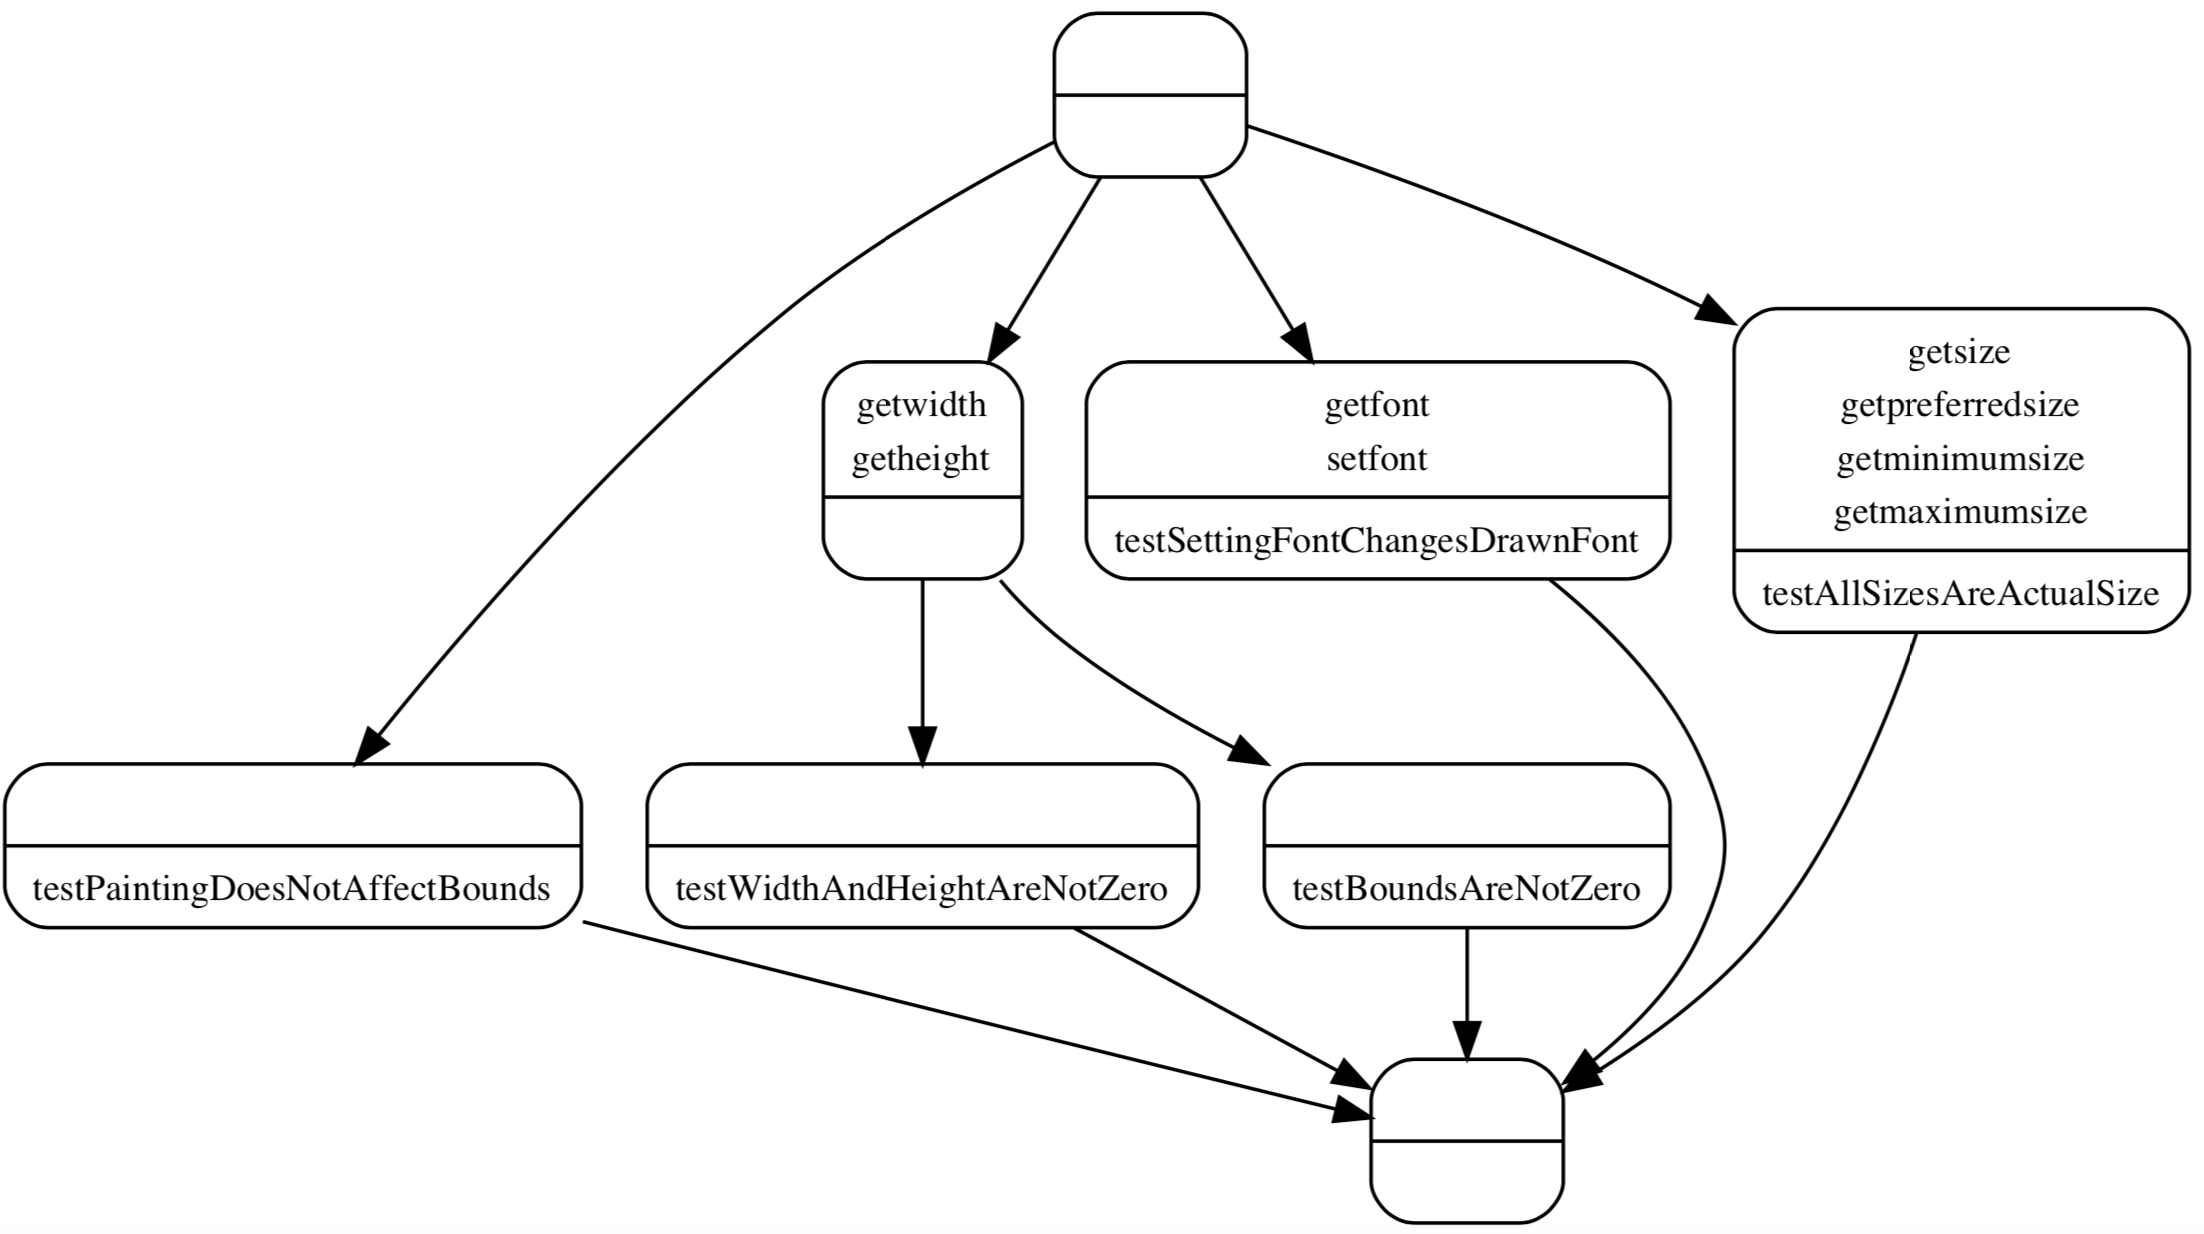
\includegraphics[scale=0.28]{figures/lattice1.png}
\caption{Concept lattice under action-CUTMethodCall code.}
\label{fig:lattice-action}
\end{subfigure}\\
\vspace{0.2cm}
\begin{subfigure}[b]{1.0\textwidth}
\centering
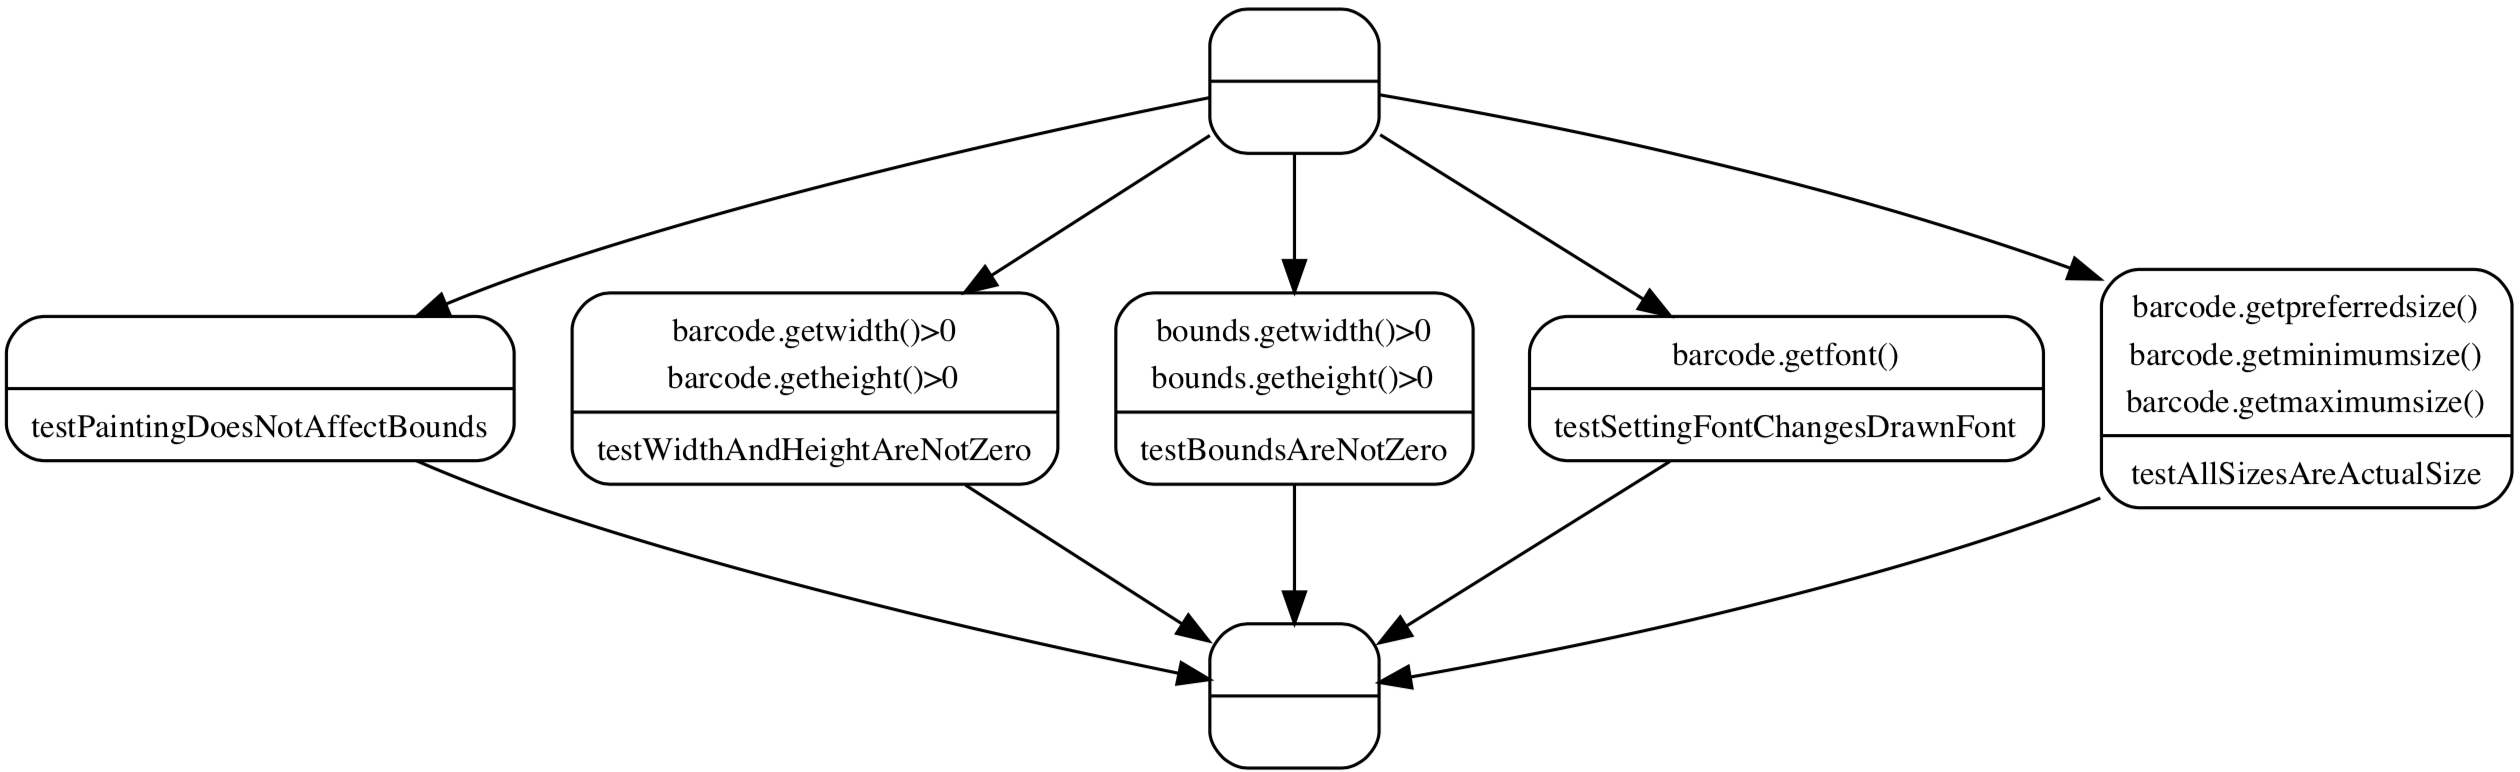
\includegraphics[scale=0.34]{figures/lattice2.png}
\caption{Concept lattice under predicate-ActualParameter code.}
\label{fig:lattice-predicate}
\end{subfigure}
\caption{Check for uniqueness via FCA}
\label{fig:fca}
\end{figure*}

The goal of Step~2 is to identify whether the current set of attributes extracted by Step~1 make the target test unique among its siblings.
%
This is accomplished using formal concept analysis (FCA) on the set of $\langle test,~attributes \rangle$ pairs from Step~1 to build a concept lattice.
%
The lattice is then analyzed to determine which, if any, of the target test's attributes, make it unique.


FCA is a data mining technique that is designed to facilitate the investigation of (implicit) relationships between a set of \emph{objects} and a set of \emph{attributes}.
%
It has been successfully used in a variety of software engineering contexts (e.g.,~\cite{tonella2004formal, tilley2005survey}).
%
In our approach, \emph{objects} are the tests and \emph{attributes} are the attributes extracted by Step~1.


As examples of a concept lattice, consider~\cref{fig:fca}.
% 
As these figures show, a concept lattice is a lattice that groups objects which share common attributes (i.e., a formal concept) and orders such groupings as a hierarchy (i.e., using subconcept\slash superconcept relations) of formal concepts~\cite{tonella2003using}.
%
A formal concept is a pair consisting of a subset of objects and a subset of attributes that is closed by Galois connection~\cite{singh2014note}.
%
For example, if the formal concept is a pair like \texttt{<objs, attrs>}, \texttt{objs} should consist of all objects that share the attributes in \texttt{attrs}, and \texttt{attrs} should consist of all attributes that are shared by the objects in \texttt{objs}.
%
The topmost node in a lattice is the concept that contains all attributes, and the bottommost node is the concept that contains all objects~\cite{atif2013mathematical}.
% 
In~\cref{fig:fca}, each lattice was built for our running example from \cref{fig:information-matcher} using different sets of attributes.


In order to simplify the presentation, lattices are shown in a reduced form, which means that each object and attribute only appears once, in the highest or lowest concept, rather than being duplicated in all super\slash sub-concepts.
%
For example, in \cref{fig:lattice-action} the concept with no objects and two attributes (\texttt{getwidth, getheight}) is a super-concept of the two lower concepts which it connects to and a super-concept of the upper objects it connects to.
%
This means that, beyond the attributes that are shown, this concept includes additional objects (\texttt{test\-Bounds\-Are\-Not\-Zero}, \texttt{test\-Width\-And\-Height\-Are\-Not\-Zero}).


To check the uniqueness of a set of attributes, we implemented an algorithm to traverse concept lattices.
%
As input, the algorithm takes a concept lattice and a given test.
% 
The algorithm then performs a depth-first search of the concept lattice to attempt to locate a concept whose objects contains only the given test.
%
If such a concept \emph{can not be} located, the approach returns to Step~1.
%
Otherwise, if such concept \emph{can be} located, the approach then extracts the subset of attributes that make the test unique.


The subset of attributes that make the test unique is extracted by looking at the reduced attributes of the identified concept.
%
If the set of reduced attributes is \emph{not} empty, it uniquely identifies the given test.
%
For example, in \cref{fig:lattice-action} \texttt{test\-Setting\-Font\-Changes\-Drawn\-Font} is uniquely identified by the attributes (\texttt{getfont, setfont}).
% 
Otherwise, if the set of reduced attributes is empty, the algorithm returns to Step~1.
%
For example, \cref{fig:lattice-action} shows that \texttt{test\-Bounds\-Are\-Not\-Zero} can not be uniquely identified based on the CUTMethodCall code and another code needs to be attempted.
%
The algorithm moves on to the next code until it finds a set of reduced attributes that can uniquely identify the test.
%
For example, while \texttt{test\-Bounds\-Are\-Not\-Zero} can not be uniquely identified in~\cref{fig:lattice-action}, \cref{fig:lattice-predicate} shows that it can be uniquely identified based on the ActualParameter code by the corresponding set of reduced attributes (\texttt{bounds.getwidth()\->\-0, bounds.getheight()\->\-0}).
% 
Finally, if all codes are tried without producing a valid set of reduced attributes, the algorithm outputs the test with an empty set of attributes.
%
For example, \texttt{test\-Painting\-Does\-Not\-Affect\-Bounds} has an empty set of reduce attributes in all subfigures in \cref{fig:fca}.


\begin{figure*}[t]
\centering
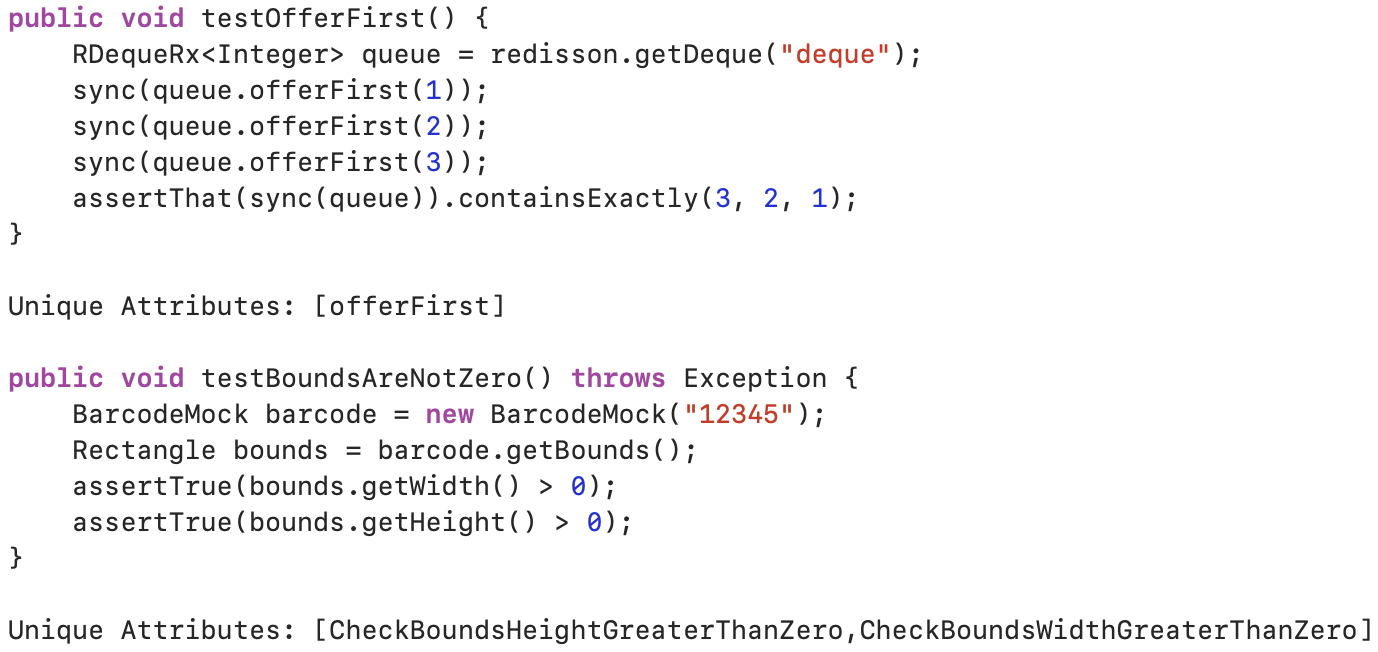
\includegraphics[scale=0.35]{figures/approach_output.png}
\caption{Examples of output of the approach.}
\label{fig:output-approach}
\end{figure*}


The unique attributes are processed by the following procedure in order to facilitate future name generation techniques (e.g., provide descriptive, human-readable test names).
%
First, the attributes are processed to remove illegal characters such as white space and special symbols (e.g., \enquote{\%} and \enquote{\#}).
%
Second, if a predicate code was used to generate the attributes, some additional manipulation is performed.
%
Instances of \enquote{$<$}, \enquote{$>$}, \enquote{$=$}, or numbers are replaced with corresponding English words like \enquote{GreaterThan} or \enquote{Zero} using a predefined lookup table.
%
If the attribute starts with \enquote{set} or \enquote{get}, it is prefixed by \enquote{When}.
%
If the attribute starts with \enquote{assert}, it is prefixed by \enquote{If}.
%
Otherwise, it is prefixed by \enquote{Check}.
%
Third, if the attribute contains Java method calls, the stop words such as \enquote{set} or \enquote{get} are removed from them.
%
Finally, the set of processed attributes is paired with the original test as the output of the approach.


As examples of unique attributes identified by the approach, consider \cref{fig:output-approach}.
%
The first test is fully named after what makes it unique.
%
The unique attribute (\texttt{offer\-First}) is identified for this test, which is fully consistent with the original name \texttt{test\-Offer\-First}.
%
The second test is partially named after what makes it unique.
%
The unique attributes (\texttt{Check\-Bounds\-Height\-Greater\-Than\-Zero,Check\-Bounds\-Width\-Greater\-Than\-Zero}) are identified for this test, which are partially consistent with the original name \texttt{test\-Bounds\-Are\-Not\-Zero}.


\subsubsection{Evaluation}
\label{sec:emp-eval-attributes}

The overall goal of empirical evaluation is to determine if our approach can match human judgment.
%
More specifically, we considered the question: \emph{Do the unique attributes identified by the approach agree with human judgment?}
%
In the context of future work, this is the most important evaluation metric.
%
If the approach can not accurately identify what makes a test unique, it can not be used for generating descriptive names.


In order to conduct the evaluation, we implemented the approach as an IntelliJ IDEA Plugin~\cite{IntelliJPlugin}.
%
IntelliJ IDEA is a full-featured IDE that can import projects from many different build systems (e.g., Maven and Gradle).
%
This gives us more flexibility in choosing applications when building our set of experimental subjects.
%
To use the plugin, developers can click on a menu item that analyzes all tests in the current project, and it could easily be extended to support other interaction mechanisms (e.g.,~run for a specific test class).

The plugin was used to gather the necessary data for performing the evaluation.
%
When running on a MacBook Pro (2.4GHz Intel i5 processor and 8GB RAM) with MacOS Mojave, Kotlin version 1.3.10, and Java version 13.0.2, the plugin analyzed all \num{31251} tests from the \num{17} projects considered in the evaluation in about \num{78} minutes (i.e., on average, \num{0.15} seconds per test).
%
We believe that this level of performance is reasonable and is fast enough to support using the tool as part of future name generation approaches.


The remainder of this section describes our experimental subjects and presents and discusses our results.

\paragraph{Experimental Subjects for Evaluation}

\begin{table*}[t]
\centering
\caption{Additional considered applications.\strut}
\begin{tabular}
{
  l
  l
  S[table-format=5.1]
  S[table-format=5.1]
}
\toprule
\multicolumn{1}{c}{\textbf{Project}} &
\multicolumn{1}{c}{\textbf{Version}} & 
\multicolumn{1}{c}{\textbf{LoC}} &
\multicolumn{1}{c}{\textbf{\# Tests}}
\\
\midrule
 Sentinel          & 10c92e6  &  79385   & 488   \\
 Jedis             & d7aba13  &  36582   & 684   \\
 Jfreechart        & 4e0a53e  &  133540  & 2176  \\
 Redisson          & 6feb33c  &  150703  & 2036  \\
 Spark             & 7551a7d  &  11956   & 310   \\
 Webmagic          & 96ebe60  &  15774   & 98    \\
\bottomrule
\end{tabular}
\label{tab:subjectsForEvaluation}
\end{table*}


As the subjects for the evaluation, we started with the \num{440} labeled tests that we used in the empirical study.
%
Because of the significant amount of human work in manually identifying what makes a test unique, it makes sense to reuse them.
%
However, because of the threat that the approach may be over-fit to these subjects, we decided to augment them.
%
To do this we first chose \num{6} additional projects from GitHub.
%
The additional projects, shown in \cref{tab:subjectsForEvaluation}, were selected using the same rational that was used for selecting the \num{11} applications from the study.
%
Then, we again sampled the set of tests in order to manage the amount of manual effort.
%
In this case, we selected \num{480} tests, \num{80} from each application.
%
Finally, using the same procedure as for the empirical study, each of the \num{480} tests was manually analyzed to identify what makes it unique among its siblings.
%
As a result, we have \num{920} tests, labeled with what makes them unique, that serve as the subjects of the evaluation.
%
A copy of this data set is publicly available~\cite{emp-data,evaluation_data}.


\paragraph{Data and Discussion}

\begin{table}[t]
\centering
\caption{Consistency rates for all projects.\strut}
\begin{tabular}
{
  l
  S[table-format=3.2]
  S[table-format=3.2]
  S[table-format=3.2]
  S[table-format=3.2]
}
\toprule
 & \multicolumn{4}{c}{\textbf{Levels of consistency (\%)}} \\
 \cmidrule(lr){2-5}

\multicolumn{1}{c}{\textbf{Project}}
& \multicolumn{1}{c}{\textbf{Equivalent}} 
& \multicolumn{1}{c}{\textbf{Approach$\boldsymbol{+}$}}
& \multicolumn{1}{c}{\textbf{Approach$\boldsymbol{-}$}} 
& \multicolumn{1}{c}{\textbf{Mismatch}}
\\
\midrule
 Barbecue             & 25.0  &  10.0 & 50.0 & 15.0   \\
 Moshi                & 35.0  &  37.5 & 12.5 & 15.0   \\
 Mockito              & 30.0  &  35.0 & 25.0 & 10.0   \\
 Guava                & 32.5  &  37.5 & 22.5 & 7.5    \\
 Guice                & 10.0  &  45.0 & 32.5 & 12.5   \\
 ExoPlayer            & 45.0  &  32.5 & 12.5 & 10.0   \\
 Scribejava           & 32.5  &  27.5 & 37.5 & 2.5    \\
 Socket.io-client     & 35.0  &  40.0 & 15.0 & 10.0   \\
 Fastjson             & 35.0  &  32.5 & 30.0 & 2.5    \\
 Picasso              & 47.5  &  12.5 & 25.0 & 15.0   \\
 Javapoet             & 12.5  &  40.0 & 30.0 & 17.5   \\
 \midrule
 Sentinel             & 25.0  &  58.8 & 12.5 &  3.7   \\
 Jedis                & 37.5  &  30.0 & 32.5 &  0.0   \\
 Jfreechart           & 42.5  &  36.3 & 21.2 &  0.0   \\
 Redisson             & 40.0  &  22.5 & 33.7 &  3.8   \\
 Spark                & 31.2  &  41.3 & 27.5 &  0.0   \\
 Webmagic             & 7.5   &  33.8 & 55.0 &  3.7   \\
 \midrule
 Overall              & 30.8  &  34.6 & 28.5 &  6.1   \\
\bottomrule
\end{tabular}
\label{tab:RQ1-1}
\end{table}


To answer the question about whether the attributes identified by the approach agree with human judgment about what makes the test unique among its siblings, it is necessary to establish a procedure for comparing the manually identified attributes with the automatically identified attributes.
%
To do this, we employed a manual review and comparison process that is similar to one used in the empirical study (see:~\cref{sec:emp-study}).
%
Together, the researchers compared the manually identified attributes with the automatically identified attributes of each test and classified the tests into one of the categories below.
%
In total, performing the \num{920} comparisons took around \num{20} hours.

\begin{enumerate}
    \item Equivalent: A test is included in the Equivalent category when 
    \begin{enumerate*}
        \item the two sets of attributes contain the same number of elements
        \item each element in one set expresses the same information as an element in the other set
    \end{enumerate*}.
    %
    For example, \texttt{test\-Offer\-First} from Redisson is included in the Equivalent category because its set of automatically identified attributes (\texttt{Offer\-First}) is the same as the manually identified attributes (\texttt{Offer\-First}).
    %
    Similarly, \texttt{test\-Serialization} from Guava is also included in the Equivalent category because its set of automatically identified attributes (\texttt{reserialize}) and its set of manually identified attributes (\texttt{reserialized}) represent the same information (i.e., \enquote{reserialize} and \enquote{reserialized} differ only in their tenses).
    
    \item Approach Plus ($\boldsymbol{+}$): A test is included in the Approach Plus category when
    \begin{enumerate*}
        \item the set of automatically identified attributes contains more elements than the set of manually identified attributes
        \item each element in the set of manually identified attributes expresses the same information as an element in the set of automatically identified attributes
    \end{enumerate*}.
    %
    For example, \texttt{client\-Id\-Reconnect} from Jedis is included in the Approach Plus category because its set of automatically identified attributes (\texttt{disconnect, connect}) is larger than its set of manually identified attributes (\texttt{disconnect}) and the element in the manually identified set (\texttt{disconnect}) is also present in the automatically generated set.
    
    \item Approach Minus ($\boldsymbol{-}$): A test is included in the Approach Minus category when
    \begin{enumerate*}
        \item the set of automatically identified attributes contains fewer elements than the set of manually identified attributes
        \item each element in the set of automatically identified attributes expresses the same information as an element in the set of manually identified attributes
    \end{enumerate*}.
    %
    For example, \texttt{test\-Exit\-Last\-Entry\-With\-Default\-Context} from Sentinel is included in the Approach Minus category because its set of automatically identified attributes (\texttt{get\-Fake\-Default\-Context, run\-On\-Context}) contains fewer elements than its set of manually identified attributes (\texttt{get\-Fake\-Default\-Context, run\-On\-Context, default\-Con\-text.get\-Cur\-Entry}) and each element in the set of manually identified attributes is also in the set of automatically identified attributes.    

    \item Mismatch: A test is included in the Mismatch category when it does not meet the definitions of any of the above categories. 
    %
    For example, \texttt{flatten\-Top\-Level} from Moshi is included in the Mismatch category because its set of automatically identified attributes (\texttt{has\-Message}) has nothing in common with the set of manually identified attributes (\texttt{"Nesting~problem."}).
\end{enumerate}


In terms of name generation, results in the first three categories are positive.
%
They indicates cases where the approach is able to identify information that relevant for generating descriptive names.
%
For tests in the Equivalent category, our approach identifies the same unique attributes as developers would, which could be directly applied to future name generation approaches.
%
For tests in the Approach Plus category, our approach identifies the same unique attributes as developers would but includes some additional information.
%
And for tests in the Approach Minus category, our approach identifies some of the same unique attributes as developers would.
%
Only in the case of the Mismatch category does the approach fail to provide useful information.


\Cref{tab:RQ1-1} presents the results of the classification process.
%
In the table, the first column shows the name of each project and the following four columns show the percentage of tests in the Equivalent, Approach Plus, Approach Minus, and Mismatch categories, respectively.
% 
The first eleven rows show the data for the \num{11} original projects, the following six rows show the data for the \num{6} additional projects, and the final row shows the averages across all tests.
%
Each row shows the calculated data for each project.
%
For example, the twelfth row shows that for the considered tests from Sentinel, the Equivalent, Approach Plus, Approach Minus, and Mismatch rates are \SI{25.0}{\percent}, \SI{\approx 58.8}{\percent}, and~\SI{\approx 12.5}{\percent},~\SI{\approx 3.7}{\percent}, respectively.


Overall, we believe the performance of the approach is positive.
%
As the last row of the table shows, the average Equivalent, Approach Plus, and Approach Minus rates are \SI{\approx 30.8}{\percent}, \SI{\approx 34.6}{\percent}, and \SI{\approx 28.5}{\percent}, respectively, while the average Mismatch rate is only \SI{\approx 6.1}{\percent}.
%
This means that in \SI{\approx 93.9}{\percent} of cases, the approach is 
\begin{enumerate*}
    \item capable of extracting information about what makes a test unique that agrees with human judgment
    \item likely to be useful in future name generation approaches since the majority of tests are named after what makes then unique
\end{enumerate*}.


While the overall performance is strong, the data shows that our approach performed noticeably better on some projects than others.
%
For example, the approach has a~\SI{0.0}{\percent} Mismatch rate on Jedis and Jfreechart, while it has a~\SI{\geq 15.0}{\percent} Mismatch rate on Picasso and Javapoet.
%
To understand the causes of the variation and to potentially identify avenues for improving the approach, we further investigated the cases in the Approach Plus, Approach Minus, and Mismatch categories.


First, for the subjects from the Mismatch category, we found that there are many cases (i.e.,~\SI{\geq 60.0}{\percent}) where the human-identified attributes were extracted using a lower-ranked code than the code used by the approach.
%
For example, for \texttt{should\-Handle\-Scheme\-Insensitive\-Case} from Picasso, the approach used a higher-ranked code \texttt{Action-Other\-Method\-Call}, but the human judgment corresponds to a lower-ranked code \texttt{Predicate-Actual\-Parameter}.
%
In these cases, if the approach were to use the lower-ranked code, it would identify the same attributes as the human rater.
%
This suggests that, while our current ordering of the codes is effective for many projects, it is not universally suitable.
%
In future work, we could investigate ways of customizing the order of code for individual projects.


Second, for the subjects from the Approach Minus category, we found that the attributes that were missing from the set of automatically identified attributes could always be found by using an additional code or codes.
% TODO[fixed] - Put the actual sets of attributes
For example, for \texttt{null\-Bitmap\-Options\-If\-No\-Resizing\-Or\-Purgeable} from Picasso, the manually identified attributes are (\texttt{no\-Resize, is\-Null()}) and the automatically identified attributes are (\texttt{no\-Resize}).
%
The missing attributes (\texttt{is\-Null()}) could be identified by using the code \texttt{Predicate-Expected\-Parameter} which is lower-ranked than the code \texttt{Action-Other\-Method\-Call\-Argument} which was used to extract the automatically identified attributes.
%
This suggests that extending the approach to consider multiple codes may result in identifying attributes that more difference indicates it might be useful to extend the approach to be capable of applying multiple codes when extracting unique attributes.


Last, for the subjects from the Approach Plus category, we found that the additional attributes identified by the approach are unnecessary to uniquely identify a given test among its siblings.
%
For example, for \texttt{test\-Slow\-Request\-Mode} from Sentinel, the manually identified attributes are (\texttt{current, next\-Int}), and the automatically identified attributes are (\texttt{set\-Slow\-Ratio\-Threshold, entry\-And\-Sleep\-For, next\-Int, current}). 
%
While the automatically identified attributes do uniquely identify the test, the attributes (\texttt{set\-Slow\-Ratio\-Threshold, entry\-And\-Sleep\-For}) are unnecessary; (\texttt{current, next\-Int}) are sufficient.
%
These additional attributes are included because the approach extracts all attributes in a given category.
%
In this case, the code used by the approach is \texttt{Action-Other\-Method\-Call} and the attributes are all of the non-CUT method calls in the test.
%
In future work, we could potentially address this issue by modifying the approach to check whether subsets of attributes are sufficient to uniquely identify test (i.e., if all attributes uniquely identify a test, determine the smallest subset that is sufficient).


After both the empirical study and the automated approach of extracting unique attributes of tests are completed, we are two steps closer towards generating descriptive test names that meets with developer approval.
%
The following sections will introduce my future research plan to:
\begin{enumerate*}
    \item perform a further investigation of the test names categorized as partially named after what makes the test unique
    \item transform the unique and other attributes to descriptive names
    \item build a working prototype for an empirical evaluation 
\end{enumerate*}.

